\begin{frame}{Struttura}
\begin{columns}
\begin{column}{0.5\textwidth}
\begin{itemize}
    \item<1-> single backbone
    \item<2-> multi-backbone
    \item<3-> a tubi concentrici
\end{itemize}
\end{column}
\begin{column}{0.5\textwidth}
\only<1>{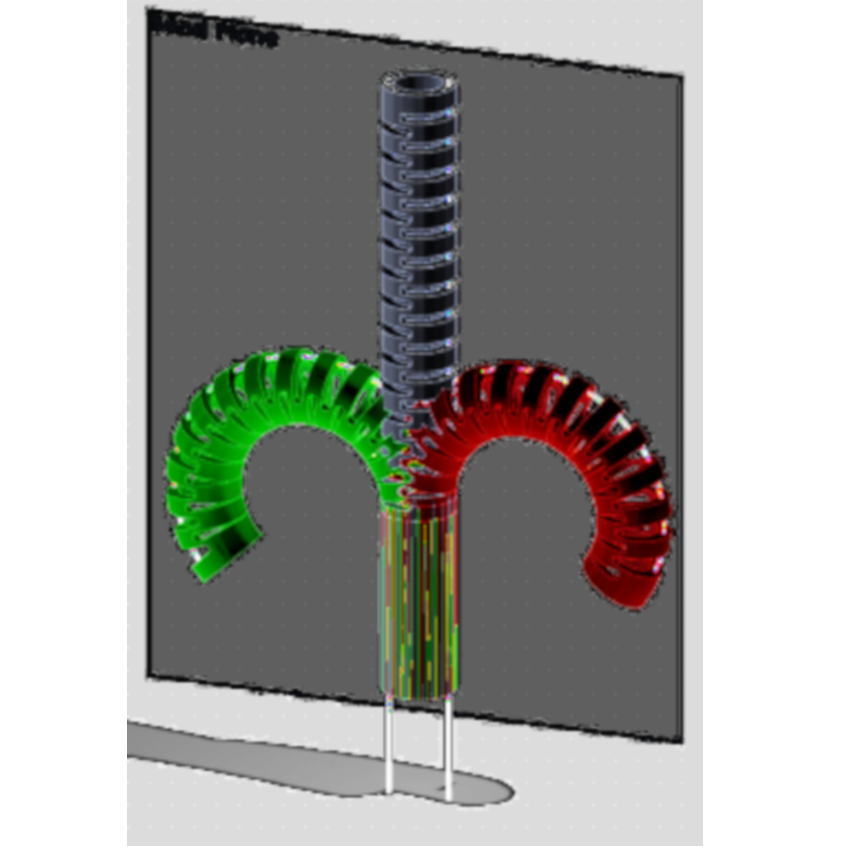
\includegraphics[height=0.7\textheight]{slide_studio/img_struttura/single_backbone.png}}
\only<2>{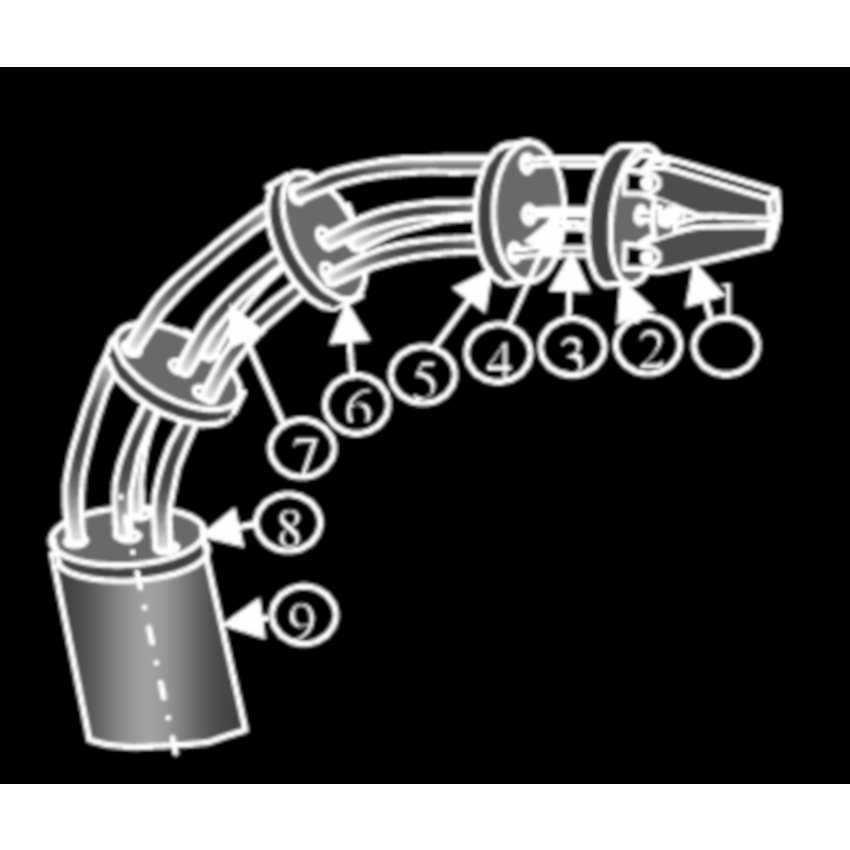
\includegraphics[height=0.7\textheight]{slide_studio/img_struttura/multi_backbone.png}}
\only<3>{\hspace*{-4em}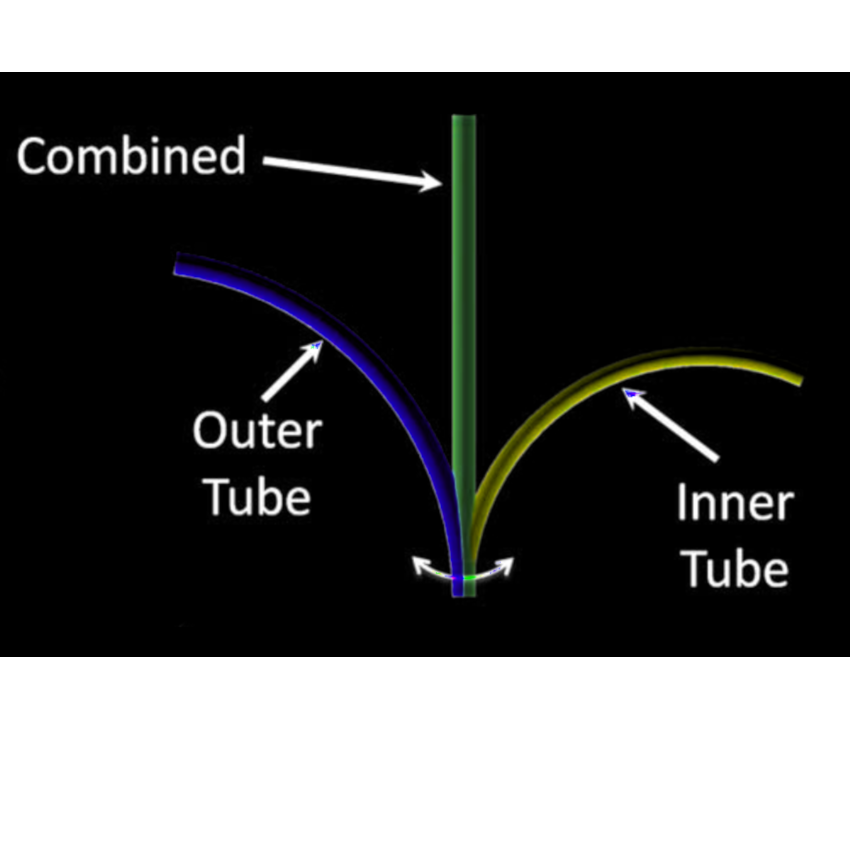
\includegraphics[height=0.7\textheight]{slide_studio/img_struttura/tubi_concentrici.png}}
\end{column}
\end{columns}

\only<1>{\Reference{Design of a new cable-driven manipulator with a large open lumen: Preliminary applications in the minimally-invasive removal of osteolysis}{Kutzer et al.}{2011}}

\only<2>{\Reference{Snake-Like Units Using Flexible Backbones and Actuation Redundancy for Enhanced Miniaturization}{Kutzer et al.}{2011}}

\only<3>{\BReference{Design and Control of Concentric-Tube Robots}{Dupont et al.}{2010}}

\note{
Single backbone $\to$ struttura elastica centrale, fa passare trasmissione, attuazione e strumenti.

Multi-backbone $\to$ elementi elastici paralleli ma vincolati. [Spiega figura: tirando 2 su 3 backbone secondarie, muovi il manipolatore in ogni direzione].

Tubi concentrici $\to$ tubi pre-curvati uno dentro l'altro. La base di ognuno viene ruotata e traslata assialmente per controllare la forma del robot. 
}
\end{frame}

\begin{frame}{Struttura}
\begin{columns}
\begin{column}{0.5\textwidth}
Solitamente composto da due componenti separate:
\begin{itemize}
    \item<2-> parte prossimale 
    \item<3-> parte distale
\end{itemize}
\end{column}
\begin{column}{0.5\textwidth}
{\centering 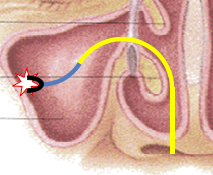
\includegraphics[height=0.5\textheight]{slide_studio/img_struttura/distal_proximal.png}}
\end{column}
\end{columns}

\note{
Può essere diviso in parte prossimale (raggiunge luogo operazione) e distale (effettua operazione).
}

\end{frame}